\section{Fuge in g-moll, BWV 861, T.~24ff}

Fast hätten wir bei unseren Analysen im Unterricht diese Fuge ausgelassen, da sie -- wahrscheinlich spätestens seit den Analysen von Erwin Ratz -- als Paradebeispiel für die Form von Bach Fugen verwendet wurde.

\begin{quote}
"<Dem Schema am nächsten steht die \emph{g-moll Fuge} des ersten Bandes.">\autocite[80f]{ratz:formenlehre}
\end{quote}

Wir wollten aber durch eigene Analysen herausfinden, warum diese Fuge als Lehrbeispiel so gut geeignet ist.
Unsere Untersuchungen haben ergeben, dass dies wahrscheinlich deshalb so ist, weil die Durchführungen sehr regelmässig aufgebaut sind und einem klaren Tonartenplan folgen\footnote{1.~Durchführung in \emph{g-moll}, 2.~Dfg. in \emph{B-dur}, 3.~Dfg. in \emph{c-moll}, 4. und 5.~Dfg. wieder in \emph{g-moll}}.
Ausserdem geht die 2.~Durchführung noch einmal, fast wie in der Exposition, durch alles Stimmen, abgesehen davon, der 4.~Themeneinsatz in T.~17 in der Tenorlage hier erneut als Basseinsatz erklingt.
Ein weiterer Punkt wäre, dass diese \emph{Fuga à 4 voci} erst recht spät in der 2.~Durchführung ab Takt 15 tatsächlich vierstimmig ist und vorher maximal drei Stimmen erklingen, was vorallem in der Exposition einer vierstimmigen Fuge etwas überrascht.

Eher untypisch ist bei dieser Fuge hingegen, dass zwischen den Durchführungen keine regelmässigen Sequenzen komponiert sind, sondern nur Orgelpunkte, Kadenz-Modelle und \emph{harmonische Sequenzen}.
Erst am Ende der Fuge zwischen den beiden letzten Durchführungen, beide in \emph{g-moll}, erklingt eine regelmässige Sequenz die mit drei Sequenzgliedern sogar relativ lang ist.
Durch die besondere ausarbeitung Bachs der Dissonanzen und Verzierungen in dieser Romanesca-Sequenz\index{Romanesca} sollen im folgenden genauer untersucht werden.
In Abbildung~\ref{fig:bwv681-original} das Notenbeispiel dazu.

\begin{figure}[htbp]
	\centering
	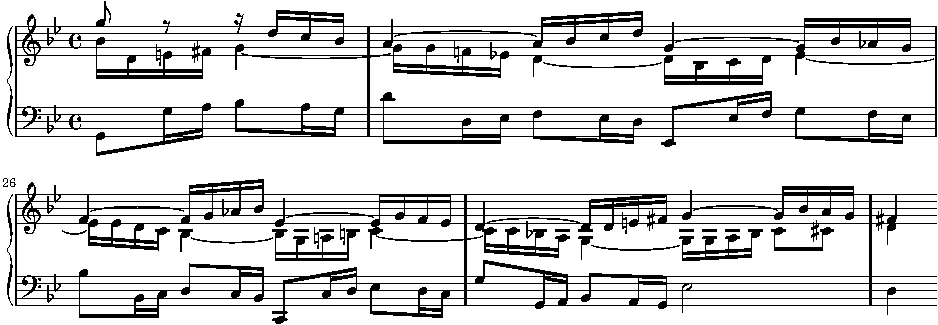
\includegraphics{lilypond/g-moll/render/original}
	\caption{Fuge in g-moll, BWV~861, T.~24ff}
	\label{fig:bwv681-original}
\end{figure}

Um einen Ausgangpunkt für weitere Analysen zu haben sei in Abbildung~\ref{fig:bwv681-romanesca-standard} die Standard Romanesca über Bachs Bass mit der üblichen 4--3 9--8 Bezifferung gegeben.

\begin{figure}[htbp]
	\centering
	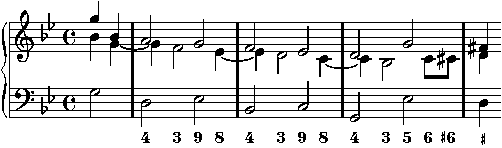
\includegraphics{lilypond/g-moll/render/romanesca-standard}
	\caption{Typische Romanesca mit 3-2-consecutive in den Oberstimmen}
	\label{fig:bwv681-romanesca-standard}
\end{figure}

Lorem ipsum dolor sit amet, consectetur adipisicing elit, sed do eiusmod tempor incididunt ut labore et dolore magna aliqua. Ut enim ad minim veniam, quis nostrud exercitation ullamco laboris nisi ut aliquip ex ea commodo consequat. Duis aute irure dolor in reprehenderit in voluptate velit esse cillum dolore eu fugiat nulla pariatur. Excepteur sint occaecat cupidatat non proident, sunt in culpa qui officia deserunt mollit anim id est laborum.

\begin{figure}[htbp]
	\centering
	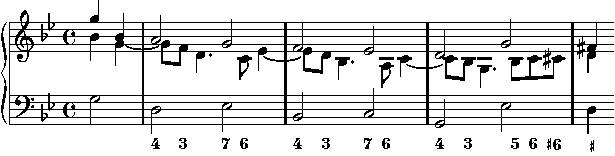
\includegraphics{lilypond/g-moll/render/romanesca-vorhalte}
	\caption{Bachs Harmonisierung der Romanesca-Sequenz in der Fuge in g-moll, BWV~861, T.~24ff}
	\label{fig:bwv681-vorhalte}
\end{figure}

Lorem ipsum dolor sit amet, consectetur adipisicing elit, sed do eiusmod tempor incididunt ut labore et dolore magna aliqua. Ut enim ad minim veniam, quis nostrud exercitation ullamco laboris nisi ut aliquip ex ea commodo consequat. Duis aute irure dolor in reprehenderit in voluptate velit esse cillum dolore eu fugiat nulla pariatur. Excepteur sint occaecat cupidatat non proident, sunt in culpa qui officia deserunt mollit anim id est laborum.
